\section{Long short-term memory} 

\textit{Long short-term memory} (LSTM) were proposed (1997) by Hochreiter and Schmidhuber\cite{lstm} as a novel network 
structure to address the vanishing gradient problem, which was first studied by Hochreiter (1991) in his diploma 
thesis, a milestone of deep learning.

The idea behind this structure is to enforce a constant error flow, that is to say, to have constant gradient norm, 
thus preventing the gradient to vanish. This is done by introducing special types of neurons called \textit{memory 
cells} and \textit{gate units}. As we can see by looking at figure \ref{lstm_neuron}, a memory cell is essentially a 
neuron with a self connection with unitary weight, whose input and output are managed by two multiplicative neurons: 
the gate units.


\tikzstyle{nn_style}=[->,shorten >=1pt,auto,node distance=1.5cm,
  thick,
  neuron/.style={circle,fill=white!50,node distance=1cm,draw,minimum size=0.7cm,font=\sffamily\normalsize},
  missing/.style={circle,font=\sffamily\Large,node distance=0.95cm},
  label/.style={node distance=1.2cm,rectangle,fill=white!50,draw=none,minimum size=0.7cm,font=\sffamily\normalsize},
  layer/.style={rectangle,fill=white!50,draw,minimum width=0.8cm,font=\sffamily\Large},
  loopStyle/.style={in=120,out=60, distance=2.5cm},
  weight/.style = {above,sloped,pos=0.3},]
\begin{figure}[h]
  \centering
  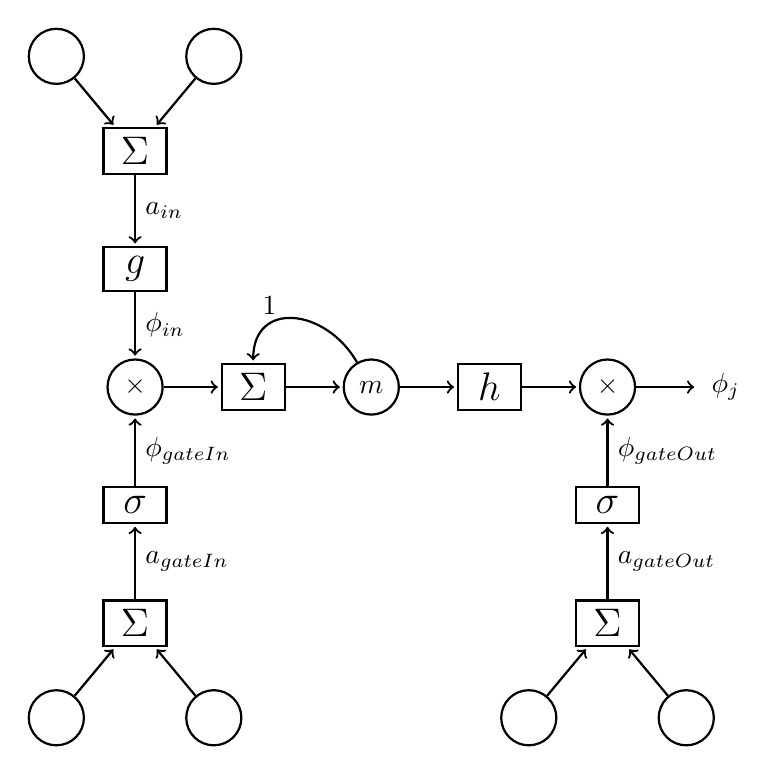
\begin{tikzpicture}[nn_style]

    %horizontal line
    \node[neuron]	(c1)       					{$\times$};
    \node[layer] 	(s_mem)	[right of=c1,	node distance=1.5cm] 	{$\Sigma$};
    \node[neuron]	(mem)	[right of=s_mem,node distance=1.5cm]	{$m$};
    \node[layer] 	(h)	[right of=mem,	node distance=1.5cm] 	{$h$};
    \node[neuron]	(c2)	[right of =h,	node distance=1.5cm]	{$\times$};
    \node[label]  	(out)	[right of=c2,	node distance=1.5cm]	{$\phi_j$};
    
    \path[->] (c1) 	edge []   (s_mem)
	      (s_mem) 	edge []   (mem)
	      (mem) 	edge []   (h)
	      (h) 	edge []   (c2)
	      (c2) 	edge []   (out);
    
    %loop	     
    \path[->] (mem) edge [loop, in=90,out=120, distance=0.8cm, anchor=south ] node [align=center, pos=0.7] 
 {$1$} (s_mem);

    
    %above inputs
    \node[layer] 	(g)	[above of=c1,	node distance=1.5cm] 	{$g$};
    \node[layer] 	(s_in)	[above of=g,	node distance=1.5cm] 	{$\Sigma$};
    \node[missing]	(i2)	[above of=s_in, node distance=1.2cm]	{$\hdots$};
    \node[neuron]	(i3)	[right of=i2, 	node distance=1cm]	{};
    \node[neuron]	(i1)	[left of=i2, 	node distance=1cm]	{};

    
    \path[->] (s_in) 	edge [anchor=west]	node[]{$a_{in}$}	(g)
	      (g) 	edge [anchor=west]   	node[]{$\phi_{in}$}	(c1)
	      (i1)	edge []   					(s_in) 
      	      (i3)	edge []   					(s_in);
      	      
      	      
    %below gate input unit
    \node[layer] 	(sig_in)	[below of=c1,		node distance=1.5cm] 	{$\sigma$};
    \node[layer] 	(s_gate_in)	[below of=sig_in,	node distance=1.5cm] 	{$\Sigma$};
    \node[missing]	(gi2)		[below of=s_gate_in, 	node distance=1.2cm]	{$\hdots$};
    \node[neuron]	(gi3)		[right of=gi2, 		node distance=1cm]	{};
    \node[neuron]	(gi1)		[left of=gi2, 		node distance=1cm]	{};

    
    \path[->] (s_gate_in) 	edge [anchor=west]	node[]{$a_{gateIn}$}	(sig_in)
	      (sig_in) 		edge [anchor=west]	node[]{$\phi_{gateIn}$} 	(c1)
	      (gi1)		edge []   (s_gate_in) 
      	      (gi3)		edge []   (s_gate_in);
      	      
      	      
    %below gate output unit
    \node[layer] 	(sig_out)	[below of=c2,		node distance=1.5cm] 	{$\sigma$};
    \node[layer] 	(s_gate_out)	[below of=sig_out,	node distance=1.5cm] 	{$\Sigma$};
    \node[missing]	(go2)		[below of=s_gate_out, 	node distance=1.2cm]	{$\hdots$};
    \node[neuron]	(go3)		[right of=go2, 		node distance=1cm]	{};
    \node[neuron]	(go1)		[left of=go2, 		node distance=1cm]	{};

    
    \path[->] (s_gate_out) 	edge [anchor=west]	node[]{$a_{gateOut}$}	   (sig_out)
	      (sig_out) 	edge [anchor=west]	node[]{$\phi_{gateOut}$}   (c2)
	      (go1)		edge []						   (s_gate_out) 
      	      (go3)		edge []						   (s_gate_out);

\end{tikzpicture}
\caption{Memory cell and gate units of LSTM network}
\label{lstm_neuron}
\end{figure}

The memory cell and the gate units behave accordingly to the following formulae:

\begin{equation}
\phi_{gateIn_j}(t)\defeq \sigma(\sum_u w_{gateIn_j,u}\cdot\phi_u(t-1))
\end{equation}
\begin{equation}
\phi_{gateOut_j}(t)\defeq \sigma(\sum_u w_{gateOut_j,u}\cdot\phi_u(t-1))
\end{equation}
\begin{equation}
\phi_{In_j}(t)\defeq g(\sum_u w_{In_j,u}\cdot\phi_u(t-1))
\end{equation}
\begin{equation}
 m(t)\defeq \phi_{In_j}\cdot\phi_{gateIn_j}+1\cdot m(t-1)
\label{mem_update}
\end{equation}
\begin{equation}
 \phi_j\defeq h(m(t))\cdot \phi_{gateOut_j}
\end{equation}

As we can see from equation \ref{mem_update}, the value of the memory cell $m(t)$ remains constant as long as the input 
gate doesn't ``open'' causing a ``write'' operation. Similarly the output of the memory cell, which is connected with 
the other neurons of the network, is controlled by an output gate: the memory will have a non zero output only if the 
output gate opens, which we could call a  a ``read'' operation. As for constant error flow it is ensured because the 
memory cell has only a self-loop with unitary weight.

Memory cells, guarded by gate units can be employed in networks with different topology alongside traditionally 
input, output and hidden units. Another way to look at this kind of architecture is to think of memory cells as units 
able to store one bit of information, even for long periods of time, hence able to learn distant time correlations 
between inputs.







